% \begin{figure}[]  % Side caption figure
%     \begin{minipage}{0.25\textwidth}
%     \includegraphics[width=\textwidth]{figures/vertical.png} % Replace with your image
%     \end{minipage}
%     \hfill
%     \begin{minipage}{0.73\textwidth}
%     \caption{The figure shows the projection of prediction errors for two-dimensional states over a horizon of $\horizon = 2$. The left figure illustrates the projection on the $(R^1, R^2)$ axes (e.g., $k=1$), and the right figure displays the projection on the $(R^3, R^4)$ axes (e.g., $k=2$). This figure provides a comparison between the inflating hypercubes for a confidence level $\delta \in (0,1)$, generated by the PCA approach (red hypercubes) and the method proposed in \cite{hashemi2024statistical} (green hypercubes). It clearly demonstrates the superior accuracy of the PCA technique compared to the other method. The principal axes for $k=1,2$ are $(r^1, r^2)$ and $(r^3, r^4)$, respectively.}
%     \label{fig:compy}
%     \end{minipage}
% \end{figure}
\begin{figure}
    \centering
    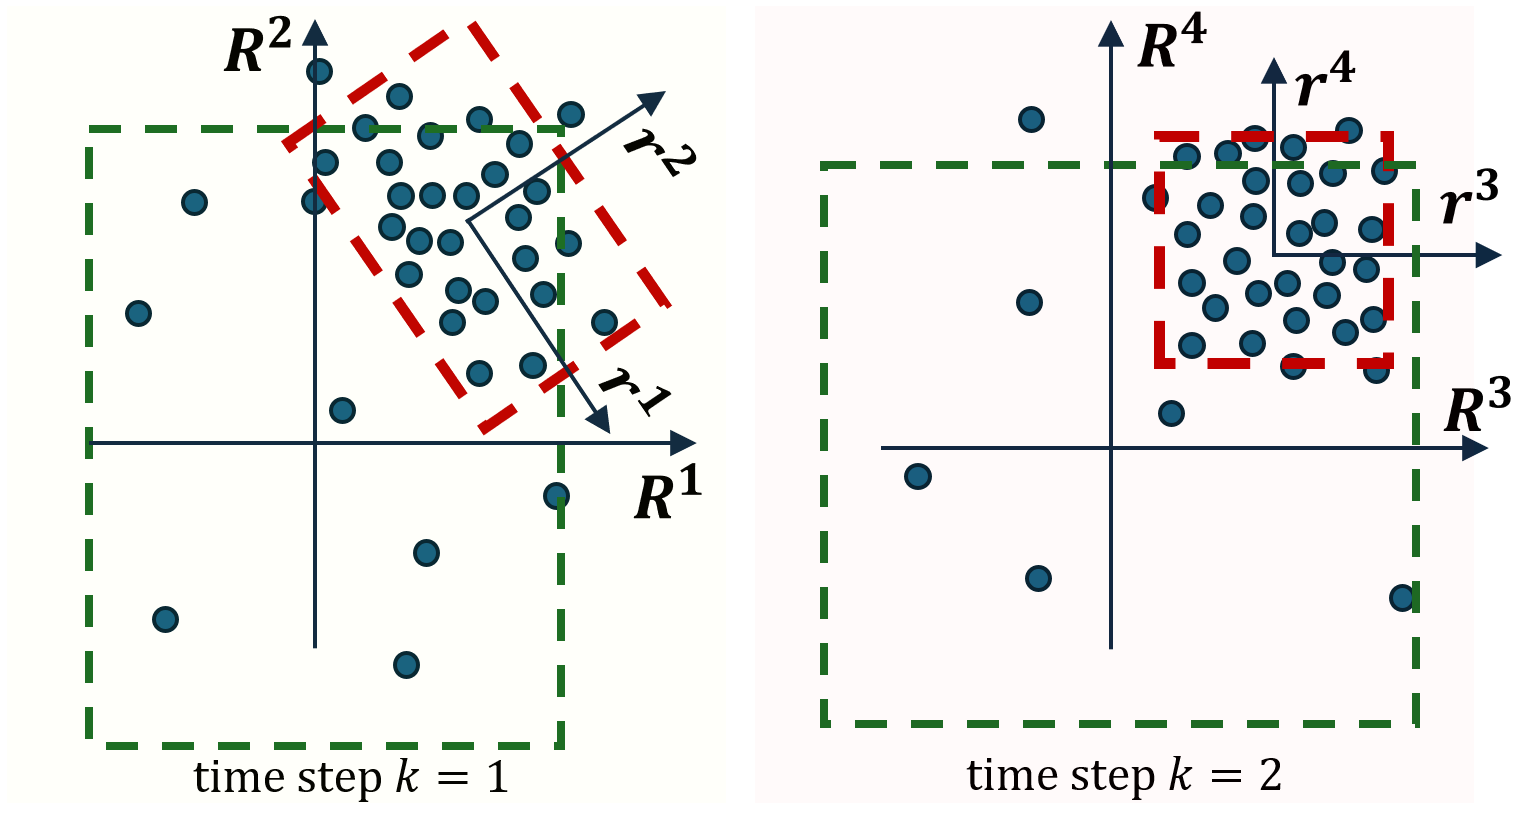
\includegraphics[width=0.45\linewidth]{figures/PCA_mtivation3.png}
    \vspace{-4mm}
    \caption{The figure shows the projection of prediction errors for two-dimensional states over a horizon of $\horizon = 2$. The left figure illustrates the projection on the $(R^1, R^2)$ axes (e.g., $k=1$), and the right figure displays the projection on the $(R^3, R^4)$ axes (e.g., $k=2$). This figure provides a comparison between the inflating hypercubes for a confidence level $\delta \in (0,1)$, generated by the PCA approach (red hypercubes) and the method proposed in \cite{hashemi2024statistical} (green hypercubes). It clearly demonstrates the superior accuracy of the PCA technique compared to the other method. The principal axes for $k=1,2$ are $(r^1, r^2)$ and $(r^3, r^4)$, respectively.}
    \label{fig:compy}
    \vspace{-4mm}
\end{figure}
\navidd{Principal Component Analysis (PCA) is a mathematical technique used to identify the principal directions of variation in a dataset. Given a dataset of $L$ data points, \( x_i \in \mathbb{R}^{n}, i\in[L]  \), PCA estimates the covariance matrix, $\Sigma \succeq 0, \Sigma \in \mathbb{R}^{n\times n}$ of data points $x_i, i\in[L]$. The eigenvectors of \( \Sigma \), known as \textbf{principal components}, define the directions along which the data exhibits the highest variance, while the corresponding eigenvalues quantify the magnitude of variance along each direction. These principal components form an orthonormal basis that aligns with the natural structure of the data, providing key insights into its intrinsic geometric properties.}

The authors in \cite{hashemi2024statistical} use the function in \eqref{eq:Rmax} to define the residual $\rho$ and compute the corresponding inflating hypercube $\delta X$. 
% They also treat the coefficients $\alpha_j, j \in [n\horizon]$ as some tunable parameters and train them to ensure that the inflating hypercube is minimized. 
% The authors in \cite{hashemi2024statistical} utilize the measurable function, introduced in \eqref{eq:Rmax} to define the residual and compute for its corresponding inflating hypercube $\delta X$. They also assume the coefficients $\alpha_j, j\in[n\horizon]$ as some scaling factors, where they train them to make it certain the inflating hypercube is as small as possible. 
\navid{However, their technique imposes two conservative constraints. First, the center of the hypercube is always located at the origin. Second,
the edges of the hypercube are restricted to be aligned with the direction of the trajectory state components.}

To address these limitations, we propose \navid{an adjustment on the definition of the residual $\rho$ in equation \eqref{eq:Rmax},} that enables us to overcome these issues. We integrate the concepts of Conformal Inference (CI) and Principal Component Analysis (PCA) in our new definition for the residual. This approach provides the principal axes as the orientation of inflating hypercube and noticeably reduces its size. In other words, our approach enhances the accuracy of conformal inference by manipulating the coordinate system, inspired by PCA. However, in the context of CI, altering the coordinate system has also been addressed in other works, such as \cite{tumu2024multi,sharma2024pac}.

To obtain the principal axes, given the simulated trajectories from the training dataset $\trajsim_{\statee_{0,i}} \in \traindataset, i\in [|\traindataset|]$, for each segment $q\in[N]$, we use the trajectory segment $\trajsimseg{q}_{\statee_{0,i}}$ and its corresponding surrogate model $\overallf_q(\statee_{0,i}; \theta_q)$ to compute the corresponding set of prediction errors. Specifically, for each segment $q\in [N]$ and data index $i\in[|\traindataset|]$, we collect: 
\begin{equation}
\PEsimseg{q}_i = \left[ \errsim{t_q n+1}_i, \errsim{t_q n+2}_i, \ldots, \errsim{(t_q+T_q)n}_i \right]
\end{equation}
% \[
% \PEsimseg{q}_i = \left[ \errsim{t_q n+1}_i, \errsim{t_q n+2}_i, \ldots, \errsim{(t_q+T_q)n}_i \right],
% \]
and approximate the average and covariance as follows:
\begin{equation}
\navid{\overline{\PE}^{q}} = \frac{\sum_{i=1}^{|\traindataset|} \PEsimseg{q}_i}{|\traindataset|} , \ \Sigma^q = \frac{\sum_{i=1}^{|\traindataset|} \left(\PEsimseg{q}_i \!\!- \overline{\PE}^{q}\right)^\top \left(\PEsimseg{q} \!\!- \overline{\PE}^{q}\right)}{|\traindataset|}.    
\end{equation}
% \[
% \begin{aligned}
% &\overline{\PE}^{q} = \frac{1}{|\traindataset|} \sum_{i=1}^{|\traindataset|} \PEsimseg{q}_i, \\
% &\Sigma^q = \frac{1}{|\traindataset|}\sum_{i=1}^{|\traindataset|} \left(\PEsimseg{q}_i \!\!- \overline{\PE}^{q}\right)^\top \left(\PEsimseg{q} \!\!- \overline{\PE}^{q}\right).
% \end{aligned}
% \]
% We then apply spectral decomposition to obtain the array of eigenvectors $\eigvecseg{q} \in \mathbb{R}^{T_q n \times T_q n}$ of the covariance matrix $\Sigma^q_i$. We finally map all the prediction errors $\errsim{j}_i , j\in[n\horizon], i \in [|\traindataset|]$ on the principal axes, which are the columns of $\eigvecseg{q}$, and we denote them with $\errmapsim{j}_i$ as,
We then apply spectral decomposition on the covariance matrix $\Sigma^q$ to obtain the array of eigenvectors $\eigvecseg{q} \in \mathbb{R}^{T_q n \times T_q n}$. Here, the principal axes for the trajectory segment $q \in [N]$ are centered on $\overline{\PE}^{q}$, and are aligned with the eigenvectors $\eigvecseg{q}_\ell, \ell \in [T_q n]$, which are the $\ell$-th columns of the matrix $\eigvecseg{q}$.
% Here, the principal axes for the trajectory segment $q \in [N]$ are aligned with the eigen-vectors $\eigvecseg{q}_\ell , \ell \in[T_qn]$ that are the $\ell$-th columns in the matrix $\eigvecseg{q}$ and centered on $\overline{\PE}^{q}$. 

Given the initial state, $\statee_0 \sim \mathcal{W}$, assume a trajectory $\statee_1, \ldots, \statee_\horizon$ that is not necessarily sampled from $\distzero$ and also is not necessarily a member of the training dataset. For any segment $q \in [N]$ of this trajectory, we map its vector of prediction errors $\PE^q = \left[ R^{t_q n+1}, R^{t_q n+2}, \ldots, R^{(t_q+T_q)n} \right]$ to the principal axes. We do this with a linear map, as, 
\begin{equation}\label{eq:PCAerror}
\left[ r^{t_q n+1},r^{t_q n+2}, \ldots, r^{(t_q+T_q)n} \right] = \transpose{\eigvecseg{q}} (\PE^q - \overline{\PE}^{q}),
\end{equation} 
and utilize the parameters $r^j,\ t_q n+1\leq j \leq (t_q+T_q)n$ to define the residual. Collecting the mapped prediction errors for all segments $q\in[N]$, we propose our definition for residual as follows:
\begin{equation}\label{eq:PCAres}
    \rho:=  \max \left(\  \frac{|r^1|}{\omega_1} ,\  \frac{|r^2|}{\omega_2} ,\  \ldots \ , \  \frac{|r^{n\horizon}|}{\omega_{n\horizon}}\ \right)
\end{equation}
where the scaling factors $\omega_j , j \in [n\horizon]$ are the maximum magnitude of parameters $r^j_i , i\in |\traindataset|$, that are obtained from the training dataset. In other words,
\begin{equation}
\omega_j = \max( |r^{j}_1|,\  |r^{j}_2|,\  \ldots,\  |r^{j}_{|\traindataset|}|  ),\ \  j \in[n\horizon]. 
\end{equation}
 % In this definition, the hyperparameters $\eigvecseg{q}, \overline{\PE}^q, q\in[N]$ and the scaling factors $\omega_j, j\in[n\horizon]$ are all generated via training dataset, $\traindataset$. 

% Subsequently, we map all the prediction errors $\errsim{j}_i$, where $t_q n+1\leq j \leq (t_q+T_q)n,\  i \in [|\traindataset|]$ onto the principal axes, which are aligned with the columns of $\eigvecseg{q}$, and centered on $\overline{\PE}^{q}$. We denote these linearly mapped prediction errors as $\errmapsim{j}_i$, and this linear map is given by:
% \begin{equation}\label{eq:PCAerror}
% \resizebox{\linewidth}{!}{$
% \left[ \errmapsim{t_q n+1}_i,\! \errmapsim{t_q n+2}_i \!\!\!\!\!\!\!\!\!\!, \ldots, \errmapsim{(t_q+T_q)n}_i \right] \!= \!\transpose{\eigvecseg{q}} \!(\PEsimseg{q}_i \!- \overline{\PE}^{q}).
% $}
% \end{equation} 
% Unlike the prediction errors, $\errsim{j}_i$ that are positive, their mapped version $\errmapsim{j}_i$ can also obtain negative values. Thus, we utilize its absolute values in our new definition for residual. Collecting the mapped prediction errors for all segments $q\in[N]$, we propose our definition for residual as follows:
% \[
% \resmapsim_i = \max( \frac{|\errmapsim{1}_i|}{\omega_1} , \frac{|\errmapsim{2}_i|}{\omega_2} , \ldots, \frac{|\errmapsim{n\horizon}_i|}{\omega_{n\horizon}})
% \]
% where the scaling factors $\omega_j , j \in [n\horizon]$ are obtained from training dataset, as the maximum level of error for that trajectory component. In other words,
% \[
% \omega_j = \max( |\errmapsim{j}_1|,\  |\errmapsim{j}_2|,\  \ldots,\  |\errmapsim{j}_{|\traindataset|}|  ),\ \  j \in[n\horizon]. 
% \]
% We also expand our residual definition for a general trajectory $\statee_0, \statee_1, \ldots, \statee_{\horizon}$ that is not necessarily sampled from $\distzero$, as,
% \begin{equation}\label{eq:PCAres}
%     \rho:=  \max \left(\  \frac{|r^1|}{\omega_1} ,\  \frac{|r^2|}{\omega_2} ,\  \ldots \ , \  \frac{|r^{n\horizon}|}{\omega_{n\horizon}}\ \right)
% \end{equation}
% where $r^j , j\in[n\horizon]$ is the proposed linear map of prediction error $R^j$ using the matrices $\eigvecseg{q}, \overline{\PE}^q,\ q\in[N]$. Here, the matrices $\eigvecseg{q}, \overline{\PE}^q$ and the scaling factors $\omega_j, j\in[n\horizon]$ are all generated via training dataset, $\traindataset$. 

Although we use the training dataset $\traindataset$ to determine hyperparameters, $\eigvecseg{q}$, $\overline{\PE}^q$, and $\omega_j$ for defining the residual, reusing $\traindataset$ to generate the inflating hypercube with robust conformal inference violates CI rules. Thus, in order to generate the inflating hypercube, we first sample a new i.i.d. set of trajectories from the training environment $\distzero$, which we denote as the calibration dataset.
\begin{definition}[Calibration Dataset] The calibration dataset $\calibdataset$ is defined as:
\begin{equation}
\calibdataset \!=\! 
\left\{ 
    \left(\statee_{0,i}, \rho_i \right) \middle|
    \begin{array}{l}
        \statee_{0,i}\sim \mathcal{W}, \, \trajsim_{\statee_{0,i}} \sim \distzero,  \\
        \rho_i = \max( \frac{|r^1_i|}{\omega_1}, \ldots, \frac{|r^{n\horizon}_i|}{\omega_{n\horizon}})
    \end{array}
\right\}.
\end{equation}
\noindent Here, $\trajsim_{\statee_{0,i}}, i \in |\calibdataset|$ refers to the trajectory starting at the $i^{th}$ initial state sampled from $\mathcal{W}$, generated from $\distzero$. The parameters $r^j_i$ are also as defined in equation~\eqref{eq:PCAerror}.
% , where the hyperparameters $\eigvecseg{q}, \overline{\PE}^q, q\in[N]$, and $\omega_j, j\in[n\horizon]$ are all obtained via training dataset, $\traindataset$.
\end{definition}
% \begin{remark}
% It is worth noting that although the data points within a single trajectory may not be i.i.d., the trajectory $\trajsim_{\statee_0}$ can be treated as an i.i.d. random vector in the $\reals^{n\horizon}$-space, and subsequently the residuals are also i.i.d. This is crucial to apply robust conformal inference, which requires that the calibration set is exchangeable.
% \end{remark}

Consider sorting the i.i.d. residuals $\rho_i \sim \distzeroR$ collected in the calibration dataset $\calibdataset$ by their magnitude: $\rho_1 < \rho_2 < \ldots < \rho_{|\calibdataset|}$. Our goal is to provide a provable upper bound for the $\delta$-quantile of a residual $\rho \sim \distR$, given knowledge of a radius $\tau > 0$ such that the total variation $\tv(\distR, \distzeroR) < \tau$. In this case, robust conformal inference \cite{cauchois2020robust} suggests using the rank $\ell^*$ from equation \eqref{eq:robustrank} and selecting $\rho^*_{\delta, \tau} := \rho_{\ell^*}$ as an upper bound for the residual's $\delta$-quantile. In other words, for a residual $\rho \sim \distR$, we have $\Pr[\rho < \rho^*_{\delta, \tau}] > \delta$.

\begin{proposition}\label{prop:maxcontribution}
Assume $\rho^*_{\delta,\tau}$ is the $\delta$-quantile of $\rho \sim \distR$, computed over the residuals $\rho_i \sim \distzeroR$ from the calibration dataset $\calibdataset$ where $\tv(\distR, \distzeroR)<\tau$. For the residual $\rho=  \max \left(\  \frac{|r^1|}{\omega_1} ,\  \frac{|r^2|}{\omega_2} ,\  \ldots \ , \  \frac{|r^{n\horizon}|}{\omega_{n\horizon}}\ \right)$ sampled from the distribution $\distR$, and the trajectory division setting, $T_q, q\in[N]$, it holds that, $\Pr\left[ P(r^1,\ldots,r^{n\horizon}) = \top \right] > \delta$, where,
\vspace{-3mm}
\begin{equation}\label{eq:probguarantee}
P(r^1,\ldots,r^{n\horizon}) \!\! = \!\!\! \bigwedge_{q=1}^{N} \!\! P_q(r^{t_qn+1}\!\!\!\!\!\!\!\!\!\!\!,\ldots,r^{(t_q+T_q)n}),\ \ P_q(r^{t_qn+1}\!\!\!\!\!\!\!\!\!,\ldots,r^{(t_q+T_q)n}) \!\! :=\!\!\!\!\!\!\!\!\bigwedge_{j=t_qn+1}^{(t_q+T_q)n} \!\!\!\!\!\!\!\left(-\omega_j\rho^*_{\delta,\tau}\leq r^j \leq \omega_j\rho^*_{\delta,\tau} \right) ,
\end{equation}
\vspace{-4mm}
and $r^j$ is the mapped version of prediction errors $R^j,\ j\in [n\horizon]$ on principal axes.
\end{proposition}
\begin{proof}
The proof follows as the residual $\rho$ is the maximum of the normalized version of parameters $r^j, j\in n\horizon$ so that
\vspace{-3mm}
\begin{equation}
\rho=  \max \left(\  \frac{|r^1|}{\omega_1} ,\  \frac{|r^2|}{\omega_2} ,\  \ldots \ , \  \frac{|r^{n\horizon}|}{\omega_{n\horizon}}\ \right)\!\! \iff \!\! \bigwedge_{j=1}^{n\horizon} \left[ |r^j| \leq \rho \omega_j \right].
\end{equation}
\vspace{-3mm}\\
Now, since $\Pr[ \rho \leq \rho^{*}_{\delta,\tau} ] \geq \delta$ as well as $\rho<\rho^*_{\delta,\tau} \iff |r^j|< \rho^*_{\delta,\tau} \omega_j$ for all $j\in [n\horizon]$, we can claim that  $\Pr[ \bigwedge_{j=1}^{n\horizon} [ |r^j| \leq \rho^*_{\delta,\tau} \omega_j ]] \geq \delta$. The guarantee proposed in \eqref{eq:probguarantee} is the reformulation of this results in terms of the division setting, $T_q, q\in [N]$.    
\end{proof}
Referring to Def.~\ref{def:star}, and using the predicates $P_q(r^{t_qn+1}\!\!\!\!\!\!\!\!\!,\ldots,r^{(t_q+T_q)n}), q\in[N]$ from Proposition \ref{prop:maxcontribution} we can introduce the inflating hypercubes, $\delta X_q , q\in [N]$ as star sets. In other words, from equation \eqref{eq:PCAerror}, for any $q\in[N]$ we can compute the prediction errors as,
\begin{equation}
\PE^q = \overline{\PE}^q + \eigvecseg{q}\left[ r^{t_q n+1},r^{t_q n+2}, \ldots, r^{(t_q+T_q)n} \right]
\end{equation}
which implies $\delta X_q = \langle \overline{\PE}^q, \eigvecseg{q}, P_q(r^{t_qn+1}\!\!\!\!\!\!\!\!\!,\ldots,r^{(t_q+T_q)n}) \rangle$, and thus the concatenation of the star sets $\delta X_q$, serves as an inflating hypercube for $\PE$. \navid{Therefore, we denote the inflating hypercube of the entire trajectory by $\delta X = \langle \overline{\PE}, V, P \rangle$ where $V = \mathbf{diag}\left(V^1, \ldots, V^N\right)$ and $P = \bigwedge_{q=1}^N P_q$.} 

\navid{Finally, based on Lemma \ref{lem:inclusion_conformal}, the $\delta$-confident flowpipe on the entire \navidg{trajectory} $X$ can be obtained through the inflation of surrogate flowpipe $\bar{X}$ with the inflating hypercube $\delta X$, i.e., $X = \bar{X}\oplus \delta X$ }.
% \begin{remark}
% Unlike the method described in \cite{hashemi2024statistical}, where the inflating hypercube expands the surrogate reachset $\bar{X}$ without repositioning it, our approach first moves the surrogate reachset through vectors $\overline{\PE}^q , q\in[N]$, before inflating it. It also inflates $\bar{X}$ based on the principal components of the prediction errors (i.e, $\eigvecseg{q}, q\in[N]$). This leads to a smaller inflation and also a tighter reachable set.
% \end{remark}
% Given the proposed $\delta$-quantile $\rho^*_{\delta, \tau}$ and our definition of the residual, we can propose the following guarantee for a given residual $\rho \sim \distR$:

% \[
% \Pr\left[\bigwedge_{q=1}^{N}\left(\bigwedge_{j=t_qn+1}^{(t_q+T_q)n} \left(-\omega_j\rho^*_{\delta,\tau}\leq r^j \leq \omega_j\rho^*_{\delta,\tau} \right) \right) \right] > \delta,
% \]

% This represents an inflating hypercube $\delta X_q \subset \mathbb{R}^{n T_q}$ for any trajectory segment $q \in [N]$, aligned with the eigenvectors in $\eigvecseg{q}$ and centered on $\overline{\PE}^q$.
\vspace{-3mm}
\begin{remark}
Figure \ref{fig:compy} shows the advantage of the PCA approach by illustrating prediction errors of a $2$-dimensional state over $2$ consecutive time steps\footnote{Division setting: $\horizon =2,\  n=2,\  N=2$, and $T_1=T_2= 1$.}. This figure also provides a schematic of the inflating hypercubes generated by our residual definition and those generated by the definition proposed in \eqref{eq:Rmax}. The primary function of the vectors $\overline{\PE}^q, q\in[N]$ is to reposition the surrogate reachsets $\bar{X}_q$ to locations that require minimal inflation, and the main role of $\eigvecseg{q}$ is to further reduce the necessary level of inflation.
\end{remark}

% We will also compare the inflating hypercubes generated by our residual definition with those generated by the definition proposed in \eqref{eq:Rmax} using a simple example.

% Let's sort the i.i.d residuals $\rho_i \sim \distzeroR$ that are collected inside the calibration dataset $\calibdataset$ according to their order of magnitude, i.e, $\rho_1 < \rho_2< \ldots < \rho_{|\calibdataset|}$. Here, we are interested in a provable upper bound for the $\delta$-quantile of a residual $\rho \sim \distR$, when we are aware of a radius $\tau>0$ such that their total variation $\tv(\distR, \distzeroR) < \tau$. In this case, robust conformal inference \cite{cauchois2020robust} suggests taking the rank $\ell^*$ proposed by equation \eqref{eq:robustrank} and select $\rho^*_{\delta,\tau} := \rho_{\ell^*}$ as an upper bound for its $\delta$-quantile. In other word, for a residual, $\rho \sim \distR$ we have $\Pr[ \rho < \rho^*_{\delta,\tau}] > \delta$. 

% Given the proposed $\delta$-quantile $\rho^*_{\delta, \tau}$, and our definition for residual, for a given residual $\rho \sim \distR$, we can propose the following guarantee,
% \[
% \Pr\left[\bigwedge_{q=1}^{N}\left(\bigwedge_{j=t_qn+1}^{(t_q+T_q)n} \left(-\omega_j\rho^*_{\delta,\tau}\leq r^j \leq \omega_j\rho^*_{\delta,\tau} \right) \right) \right] > \delta,
% \]
% that for any trajectory segment $q\in[N]$, represents an inflating hypercube $\delta X_q \subset \mathbb{R}^{n T_q}$ which is aligned on the eigenvectors in $\eigvecseg{q}$, and centered on $\overline{\PE}^q$. We also compare the inflating hypercubes generated by our residual definition and the definition proposed in \eqref{eq:Rmax} using a simple example.

% We combine the notion of Conformal Inference (CI) with the popular notion of Principal Component Analysis (PCA) in our new definition for the residual. Given the simulated trajectories from the training dataset $\trajsim_{\statee_{0,i}} \in \traindataset, i\in |\traindataset|$, for every segment $q\in[N]$ we utilize the trajectory segment $\trajsimseg{q}_{\statee_{0,i}}$ and its corresponding surrogate model $\overallf_q(\statee_{0,i}\ ;\theta_q)$,  to compute for its corresponding set of prediction errors. In other words, for every segment $q\in [N]$ and the data index $i\in[ |\traindataset|]$ we collect,
% \[
% \resizebox{\linewidth}{!}{$
% \PEsimseg{q}_i = \left[ \errsim{t_q n+1}_i, \errsim{t_q n+2}_i, \ldots, \errsim{(t_q+T_q)n}_i \right], 
% $}
% \]
% and we approximate for its average, and covariance as, \vspace{-2mm}
% $$
% \begin{aligned}
% &\overline{\PE}^{\mathsf{sim},q}_i = \frac{1}{|\traindataset|}\sum_{i=1}^{|\traindataset|} \PEsimseg{q}_i, \\
% &M^q_i = \sum_{i=1}^{|\traindataset|} (\PEsimseg{q}_i - \overline{\PE}^{\mathsf{sim},q}_i)^\top (\PEsimseg{q}_i - \overline{\PE}^{\mathsf{sim},q}_i)
% \end{aligned}
% $$
% and we apply spectral decomposition to achieve the array of eigen-vectors, $\eigvecseg{q} \in \mathbb{R}^{T_q n \times T_q n}$ of the covariance matrix $M^q_i$. 